\documentclass[12pt,a4paper]{article}

% ─── Page Layout ───────────────────────────────────────────────────────────────
\usepackage[a4paper, margin=0.8in, headheight=14pt]{geometry}

% ─── Fonts (XeLaTeX) ───────────────────────────────────────────────────────────
\usepackage{fontspec}
\usepackage{unicode-math}
\setmainfont{TeX Gyre Pagella}
\setmonofont[Scale=0.88]{TeX Gyre Cursor}
\setmathfont{Latin Modern Math}

% ─── Packages ──────────────────────────────────────────────────────────────────
\usepackage{xcolor}
\usepackage{colortbl}
\usepackage{titlesec}
\usepackage{enumitem}
\usepackage{tabularx}
\usepackage{booktabs}
\usepackage{array}
\usepackage{amsmath}
\usepackage{tikz}
\usetikzlibrary{shapes.geometric, arrows.meta, positioning, calc, fit, decorations.pathreplacing, patterns}
\usepackage{tcolorbox}
\tcbuselibrary{skins, breakable}
\usepackage{hyperref}
\usepackage{fancyhdr}
\usepackage{graphicx}
\usepackage{microtype}
\hyphenpenalty=10000
\exhyphenpenalty=10000
\sloppy
\usepackage{caption}
\usepackage{setspace}
\usepackage{multirow}
\usepackage{tocloft}

% ─── Q&A helper ────────────────────────────────────────────────────────────────
\newcommand{\Q}[1]{\textbf{#1}\par\noindent\ignorespaces}

% ─── Colour Palette ────────────────────────────────────────────────────────────
\definecolor{myred}{RGB}{196,30,58}
\definecolor{mydark}{RGB}{30,30,50}
\definecolor{mygreen}{RGB}{14,120,80}
\definecolor{myteal}{RGB}{0,130,140}
\definecolor{myamber}{RGB}{180,100,0}
\definecolor{mypurple}{RGB}{100,30,160}
\definecolor{mygray}{RGB}{246,247,249}
\definecolor{mgframe}{RGB}{180,185,200}
\definecolor{watermark}{RGB}{145,150,170}
\definecolor{hdrred}{RGB}{250,232,235}
\definecolor{hdrgreen}{RGB}{220,244,233}
\definecolor{hdrteal}{RGB}{220,242,244}
\definecolor{hdramber}{RGB}{253,242,215}
\definecolor{hdrpurple}{RGB}{238,228,255}
\definecolor{hdrgray}{RGB}{238,240,245}
\definecolor{rowalt}{RGB}{250,251,253}

% ─── Section Formatting ────────────────────────────────────────────────────────
\titleformat{\section}
  {\large\bfseries\color{myred}}{\thesection.}{0.5em}{}
  [\vspace{1pt}{\color{myred}\rule{\linewidth}{0.8pt}}]
\titleformat{\subsection}
  {\normalsize\bfseries\color{myteal}}{\thesubsection}{0.5em}{}
\titlespacing*{\section}{0pt}{18pt}{7pt}
\titlespacing*{\subsection}{0pt}{11pt}{4pt}

% ─── Paragraph ─────────────────────────────────────────────────────────────────
\setlength{\parindent}{0pt}
\setlength{\parskip}{4pt}

% ─── TOC Styling ───────────────────────────────────────────────────────────────
\renewcommand{\cfttoctitlefont}{\large\bfseries\color{myred}}
\renewcommand{\cftaftertoctitle}{\par\noindent{\color{myred}\rule{\linewidth}{0.8pt}}}
\setlength{\cftbeforetoctitleskip}{0pt}
\setlength{\cftaftertoctitleskip}{6pt}
\renewcommand{\cftsecfont}{\normalsize\bfseries\color{mydark}}
\renewcommand{\cftsecpagefont}{\normalsize\bfseries\color{mydark}}
\renewcommand{\cftsecleader}{\cftdotfill{\cftdotsep}}
\setlength{\cftbeforesecskip}{7pt}
\renewcommand{\cftsubsecfont}{\small\color{mydark}}
\renewcommand{\cftsubsecpagefont}{\small\color{mydark}}
\setlength{\cftbeforesubsecskip}{3pt}
\setlength{\cftsubsecindent}{1.4em}

% ─── Table helpers ─────────────────────────────────────────────────────────────
\renewcommand{\arraystretch}{1.45}
\setlength{\tabcolsep}{6pt}
\arrayrulecolor{mydark}
\newcolumntype{B}[1]{>{\small\bfseries\raggedright\arraybackslash}m{#1}}
\newcolumntype{Y}{>{\small\raggedright\arraybackslash}X}
\renewcommand{\tabularxcolumn}[1]{m{#1}}

% ─── Header / Footer ───────────────────────────────────────────────────────────
\pagestyle{fancy}
\fancyhf{}
\fancyhead[L]{\small\color{myred}\textbf{EC402}\;\color{mydark}--- Analog Circuits}
\fancyhead[R]{\small\color{myteal}\textbf{Module 3 Notes}}
\fancyfoot[C]{\small\color{mydark}\thepage}
\fancyfoot[R]{\small\color{watermark}\textit{\copyright\ Biraj}}
\renewcommand{\headrulewidth}{0.5pt}
\renewcommand{\footrulewidth}{0.3pt}

% ─── Hyperref ──────────────────────────────────────────────────────────────────
\hypersetup{
  colorlinks=true, linkcolor=myteal, urlcolor=myteal,
  pdfauthor={Biraj Sarkar (CGEC)},
  pdftitle={EC402 --- Module 3 Notes: Oscillators, Multivibrators and Current Mirrors}
}

% ─── tcolorbox styles ──────────────────────────────────────────────────────────
\tcbset{
  tikzbox/.style={
    colback=mygray, colframe=mgframe, boxrule=0.6pt, arc=4pt,
    left=8pt, right=8pt, top=6pt, bottom=6pt,
    colbacktitle=mgframe, coltitle=mydark, fonttitle=\small\bfseries
  },
  defbox/.style={
    colback=hdrgreen, colframe=mygreen, boxrule=0.8pt, arc=4pt,
    left=9pt, right=9pt, top=6pt, bottom=6pt,
    colbacktitle=mygreen, coltitle=white, fonttitle=\small\bfseries
  },
  formulabox/.style={
    colback=hdrteal, colframe=myteal, boxrule=0.8pt, arc=4pt,
    left=9pt, right=9pt, top=7pt, bottom=7pt,
    colbacktitle=myteal, coltitle=white, fonttitle=\small\bfseries
  },
  examplebox/.style={
    colback=hdramber, colframe=myamber, boxrule=0.8pt, arc=4pt,
    left=9pt, right=9pt, top=6pt, bottom=6pt,
    colbacktitle=myamber, coltitle=white, fonttitle=\small\bfseries
  },
  masonbox/.style={
    colback=hdrpurple, colframe=mypurple, boxrule=0.8pt, arc=4pt,
    left=9pt, right=9pt, top=6pt, bottom=6pt,
    colbacktitle=mypurple, coltitle=white, fonttitle=\small\bfseries
  },
  exambox/.style={
    colback=hdrpurple, colframe=mypurple, boxrule=1pt, arc=5pt,
    left=10pt, right=10pt, top=8pt, bottom=8pt,
    colbacktitle=mypurple, coltitle=white, fonttitle=\bfseries,
    breakable, title after break={\textbf{Frequently Asked / Viva Questions (contd.)}}
  }
}
\tcbset{breakable}
\tcbset{after={\color{black}}}

% ─── TikZ styles ───────────────────────────────────────────────────────────────
\tikzset{
  block/.style={rectangle, draw=myteal, fill=hdrteal,
    text width=2.4cm, align=center, minimum height=0.95cm,
    font=\small, rounded corners=3pt, line width=0.7pt},
  redblock/.style={rectangle, draw=myred, fill=hdrred,
    text width=2.4cm, align=center, minimum height=0.95cm,
    font=\small, rounded corners=3pt, line width=0.7pt},
  sumjunc/.style={circle, draw=myamber, fill=hdramber,
    minimum size=0.62cm, font=\small, line width=0.8pt},
  arrow/.style={-Stealth, thick, color=mydark},
  redarrow/.style={-Stealth, thick, color=myred},
  line/.style={thick, color=mydark}
}

\begin{document}

% ─── Title Page ───────────────────────────────────────────────────────────────
\begin{center}
  {\LARGE\bfseries\color{myred} EC402 --- Analog Circuits}\\[5pt]
  {\normalsize\color{mydark} Semester IV \quad$\bullet$\quad 3L:0T:0P \quad$\bullet$\quad 3 Credits}\\[3pt]
  {\normalsize\color{myteal}\textbf{Module 3 Exam Notes: Oscillators, Multivibrators and Current Mirrors}}\\[3pt]
  {\small\color{mydark} CGEC \;$|$\; B.Tech ECE (2023--27) \;$|$\; \textit{Biraj Sarkar}}
\end{center}
\vspace{2pt}
\noindent{\color{myred}\rule{\linewidth}{1.5pt}}
\vspace{2pt}

\hypersetup{linkcolor=mydark}
\tableofcontents
\hypersetup{linkcolor=myteal}
\newpage

\section{Oscillator Principles and the Barkhausen Criterion}

\begin{tcolorbox}[defbox, title={Oscillator Fundamentals}]
An \textbf{oscillator} is an electronic circuit that converts direct current ($dc$) power from a supply into an alternating current ($ac$) waveform of a predetermined frequency without any external $ac$ input signal. It operates on the principle of \textbf{regenerative (positive) feedback}.
\end{tcolorbox}

\subsection{The Barkhausen Criterion for Sustained Oscillations}
For an amplifier with open-loop gain $A(s)$ and feedback network transfer function $\beta(s)$, the closed-loop transfer function with positive feedback is:
\[
A_f(s) = \frac{A(s)}{1 - A(s)\beta(s)}.
\]
A non-zero output can exist with zero input ($X_s = 0$) only if the denominator vanishes at frequency $\omega_0 = 2\pi f_0$:
\[
1 - A(j\omega_0)\beta(j\omega_0) = 0 \iff A(j\omega_0)\beta(j\omega_0) = 1.
\]

\begin{tcolorbox}[formulabox, title={The Two Barkhausen Conditions}]
For self-sustained oscillations of constant amplitude at frequency $\omega_0$:
\begin{enumerate}[leftmargin=1.5em, itemsep=3pt]
  \item \textbf{Loop Gain Magnitude Condition}: The magnitude of the loop gain must equal unity:
  \[
  |A(j\omega_0)\beta(j\omega_0)| = 1.
  \]
  \textit{Practical Design Rule}: To initiate oscillations from thermal noise, the loop gain must initially be slightly greater than unity ($|A\beta| \ge 1.05$--$1.1$). Non-linear amplitude limiting (clamping, FET/thermistor resistance) subsequently stabilizes $|A\beta| = 1$ in steady state.
  \item \textbf{Phase Condition}: The total phase shift around the feedback loop must be $0^\circ$ or an integer multiple of $360^\circ$:
  \[
  \angle A(j\omega_0)\beta(j\omega_0) = 0^\circ \quad\text{or}\quad 2\pi n \quad (n = 0, 1, 2, \dots).
  \]
  If the active amplifier provides a phase shift of $180^\circ$ (inverting stage), the feedback network must introduce an additional $180^\circ$ phase shift at frequency $f_0$.
\end{enumerate}
\end{tcolorbox}

\section{Audio-Frequency ($RC$) and Radio-Frequency ($LC$) Oscillators}

\subsection{$RC$ Phase Shift Oscillator (Audio Range: $10\,\mathrm{Hz}$--$100\,\mathrm{kHz}$)}
An inverting amplifier ($180^\circ$ phase shift) is cascaded with a three-section high-pass $RC$ ladder network. Each $RC$ section produces an average phase shift of $60^\circ$, providing the required $180^\circ$ feedback phase shift.

\begin{tcolorbox}[formulabox, title={Derivation of $RC$ Phase Shift Oscillator Frequency}]
Applying KVL to the three-mesh ladder network, the feedback transfer function $\beta(s) = V_f(s)/V_o(s)$ (with $\alpha = 1/(sRC)$) is:
\[
\beta(s) = \frac{1}{1 + 6\alpha + 5\alpha^2 + \alpha^3} = \frac{1}{1 - \dfrac{5}{\omega^2 R^2 C^2} - j\left(\dfrac{6}{\omega R C} - \dfrac{1}{\omega^3 R^3 C^3}\right)}.
\]
To satisfy the phase condition $\angle \beta = 180^\circ$, the imaginary part must vanish:
\[
\frac{6}{\omega_0 R C} - \frac{1}{\omega_0^3 R^3 C^3} = 0 \implies \omega_0^2 = \frac{1}{6 R^2 C^2} \implies f_0 = \frac{1}{2\pi R C \sqrt{6}}.
\]
Substituting $\omega_0$ into the real part:
\[
\beta(j\omega_0) = \frac{1}{1 - 5(6)} = -\frac{1}{29}.
\]
To satisfy the loop gain condition $|A_v \beta| \ge 1$, the amplifier voltage gain must satisfy:
\[
|A_v| \ge 29.
\]
For a BJT circuit with collector load $R_C = k R$, the frequency becomes $f_0 = \frac{1}{2\pi R C \sqrt{6 + 4k}}$ and $h_{fe} \ge 44.5 + 23k + 4/k$.
\end{tcolorbox}

\subsection{Wien Bridge Oscillator (Laboratory Standard: $10\,\mathrm{Hz}$--$1\,\mathrm{MHz}$)}
Uses a non-inverting amplifier ($0^\circ$ phase shift) with a series $RC$ and parallel $RC$ lead-lag bridge network:
\[
Z_s = R + \frac{1}{sC} = \frac{sRC + 1}{sC},\qquad
Z_p = R \parallel \frac{1}{sC} = \frac{R}{sRC + 1}.
\]
The feedback transfer function is:
\[
\beta(s) = \frac{Z_p}{Z_s + Z_p} = \frac{sRC}{(sRC)^2 + 3sRC + 1} = \frac{1}{3 + j\left(\omega RC - \dfrac{1}{\omega RC}\right)}.
\]

\begin{tcolorbox}[formulabox, title={Wien Bridge Oscillation Frequency and Gain Condition}]
To make the phase shift zero ($\angle \beta = 0^\circ$), the imaginary term must vanish:
\[
\omega_0 RC - \frac{1}{\omega_0 RC} = 0 \implies \omega_0 = \frac{1}{RC} \implies f_0 = \frac{1}{2\pi RC}.
\]
At resonance $\omega_0$, $\beta(j\omega_0) = 1/3$. The non-inverting amplifier gain $A_v = 1 + R_f/R_1$ must satisfy:
\[
|A_v \beta| \ge 1 \implies A_v \ge 3 \iff \frac{R_f}{R_1} \ge 2.
\]
\end{tcolorbox}

\subsection{$LC$ Resonant Tank Oscillators (RF Range: $100\,\mathrm{kHz}$--$500\,\mathrm{MHz}$)}
A general three-terminal reactive feedback network satisfies $X_1 + X_2 + X_3 = 0$:
\begin{enumerate}[leftmargin=1.5em, itemsep=3pt]
  \item \textbf{Hartley Oscillator}: Uses two inductors ($L_1, L_2$ with mutual inductance $M$) and one tuning capacitor $C$:
  \[
  L_{eq} = L_1 + L_2 + 2M,\qquad
  f_0 = \frac{1}{2\pi \sqrt{L_{eq} C}},\qquad
  A_v \ge \frac{L_1 + M}{L_2 + M}.
  \]
  \item \textbf{Colpitts Oscillator}: Uses two capacitors ($C_1, C_2$) and one inductor $L$:
  \[
  C_{eq} = \frac{C_1 C_2}{C_1 + C_2},\qquad
  f_0 = \frac{1}{2\pi \sqrt{L C_{eq}}},\qquad
  A_v \ge \frac{C_2}{C_1}.
  \]
  \item \textbf{Clapp Oscillator}: Adds a small series capacitor $C_3 \ll C_1, C_2$ in series with $L$:
  \[
  \frac{1}{C_{eq}} = \frac{1}{C_1} + \frac{1}{C_2} + \frac{1}{C_3} \approx \frac{1}{C_3} \implies f_0 \approx \frac{1}{2\pi \sqrt{L C_3}}.
  \]
  \textit{Key Advantage}: Transistor parasitic junction capacitances appear across $C_1$ and $C_2$. Since $C_3 \ll C_1, C_2$, $C_{eq}$ is determined almost exclusively by $C_3$, giving exceptional frequency stability.
  \item \textbf{Crystal Oscillator}: Employs a piezoelectric quartz crystal. Series resonant frequency $f_s = \frac{1}{2\pi\sqrt{L C}}$ (low impedance) and parallel resonant frequency $f_p = \frac{1}{2\pi\sqrt{L [C C_0/(C+C_0)]}}$ (antiresonance, high impedance). Offers $Q$-factors of $10^4$--$10^6$ and frequency stability of $\pm 1\,\mathrm{ppm}$.
\end{enumerate}

\section{Multivibrators: Astable, Monostable and Bistable}

\begin{tcolorbox}[defbox, title={Multivibrator Classification}]
Multivibrators are two-stage cross-coupled non-sinusoidal switching circuits:
\begin{itemize}[leftmargin=1.5em, itemsep=2pt]
  \item \textbf{Astable (Free-Running)}: Zero stable states; toggles continuously between two quasi-stable states, generating a periodic square wave.
  \item \textbf{Monostable (One-Shot)}: One stable state, one quasi-stable state. An external trigger pulse causes a transition to the quasi-stable state for a predetermined duration $T$.
  \item \textbf{Bistable (Flip-Flop)}: Two stable states; requires external trigger pulses to switch between states. Used for digital memory storage.
\end{itemize}
\end{tcolorbox}

\subsection{Astable Multivibrator Waveform Timing}
In a symmetrical cross-coupled BJT circuit with collector resistors $R_C$ and base resistors $R$:
\[
T_1 = R_1 C_1 \ln(2) \approx 0.693 R_1 C_1,\qquad
T_2 = R_2 C_2 \ln(2) \approx 0.693 R_2 C_2.
\]
Total period and oscillation frequency:
\[
T = T_1 + T_2 = 1.386 RC,\qquad f = \frac{1}{T} = \frac{1}{1.386 RC} \approx \frac{0.72}{RC}.
\]

\section{Current Mirrors: Topologies, $V-I$ Curves and Output Resistance}

\begin{tcolorbox}[defbox, title={Current Mirror Concept}]
A \textbf{current mirror} uses a reference current $I_{ref}$ to set an output current $I_o$ in a matched transistor. The output current can equal the reference current or be a fixed multiple of it. A high output resistance helps keep $I_o$ steady as the output voltage changes.
\end{tcolorbox}

\subsection{Basic BJT Current Mirror Analysis}
Consider two matched transistors $Q_1, Q_2$ with $Q_1$ connected as a diode ($V_{CE1} = V_{BE1} = V_{BE2}$):
\[
I_{ref} = \frac{V_{CC} - V_{BE}}{R} = I_{C1} + I_{B1} + I_{B2} = I_{C1} + \frac{2I_C}{\beta}.
\]
Assuming identical matched transistors ($I_{C1} = I_{C2} = I_o$):
\[
I_{ref} = I_o \left(1 + \frac{2}{\beta}\right) \implies I_o = \frac{I_{ref}}{1 + \dfrac{2}{\beta}} \approx I_{ref}\left(1 - \frac{2}{\beta}\right).
\]
\textbf{Finite Output Resistance ($R_o$)}: Due to the Early effect ($V_A$), $I_o$ increases slightly with output voltage $V_{CE2}$:
\[
I_o = I_{ref}\left(1 - \frac{2}{\beta}\right)\left(1 + \frac{V_{CE2} - V_{BE}}{V_A}\right),\qquad R_o = \frac{\partial V_{CE2}}{\partial I_o} \approx r_{o2} = \frac{V_A}{I_o}.
\]
\textbf{Minimum Sustainable Voltage ($V_{ON}$)}: To keep $Q_2$ in the active region, $V_{CE2} \ge V_{CE,\mathrm{sat}} \approx 0.2\,\mathrm{V}$ (or $V_{DS} \ge V_{ov} = V_{GS} - V_{th}$ for MOSFETs). Maximum usable load resistance: $R_{L,\max} = (V_{CC} - V_{ON})/I_o$.

\begin{tcolorbox}[tikzbox, unbreakable, title={Basic, Widlar and Wilson Current Mirror Topologies}]
\centering
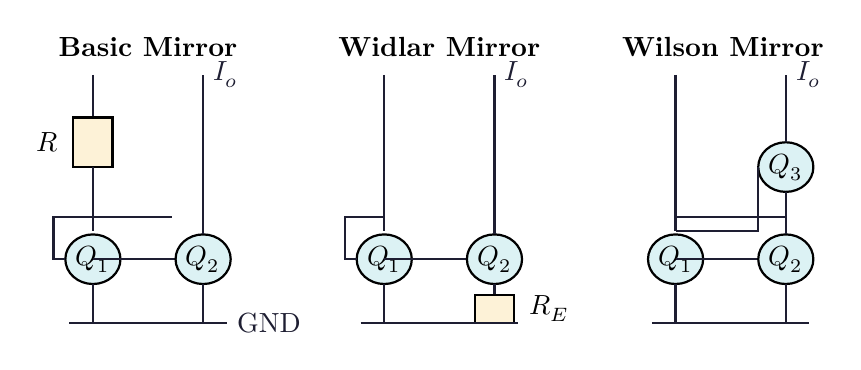
\begin{tikzpicture}[x=1cm,y=0.9cm]
  % Basic Mirror
  \node at (1.5,4.2) {\bfseries Basic Mirror};
  \draw[line] (0.8,3.8)--(0.8,3.2);
  \draw[thick,fill=hdramber] (0.55,2.5) rectangle (1.05,3.2);
  \node[left=2pt] at (0.55,2.85) {$R$};
  \draw[line] (0.8,2.5)--(0.8,1.6);
  % Q1
  \draw[thick,fill=hdrteal] (0.8,1.2) circle (0.35); \node at (0.8,1.2) {$Q_1$};
  % Diode connection
  \draw[line] (0.8,1.8)--(0.3,1.8)--(0.3,1.2)--(0.45,1.2);
  \draw[line] (0.8,1.8)--(1.8,1.8);
  % Base line
  \draw[line] (0.8,1.2)--(2.2,1.2);
  % Q2
  \draw[thick,fill=hdrteal] (2.2,1.2) circle (0.35); \node at (2.2,1.2) {$Q_2$};
  \draw[line] (2.2,1.55)--(2.2,3.8) node[right] {$I_o$};
  \draw[line] (0.8,0.85)--(0.8,0.3);
  \draw[line] (2.2,0.85)--(2.2,0.3);
  \draw[line] (0.5,0.3)--(2.5,0.3) node[right] {GND};

  % Widlar Mirror
  \node at (5.2,4.2) {\bfseries Widlar Mirror};
  \draw[line] (4.5,3.8)--(4.5,1.6);
  \draw[thick,fill=hdrteal] (4.5,1.2) circle (0.35); \node at (4.5,1.2) {$Q_1$};
  \draw[line] (4.5,1.8)--(4.0,1.8)--(4.0,1.2)--(4.15,1.2);
  \draw[line] (4.5,1.2)--(5.9,1.2);
  \draw[thick,fill=hdrteal] (5.9,1.2) circle (0.35); \node at (5.9,1.2) {$Q_2$};
  \draw[line] (5.9,1.55)--(5.9,3.8) node[right] {$I_o$};
  \draw[line] (4.5,0.85)--(4.5,0.3);
  \draw[line] (5.9,0.85)--(5.9,0.7);
  \draw[thick,fill=hdramber] (5.65,0.3) rectangle (6.15,0.7);
  \node[right=2pt] at (6.15,0.5) {$R_E$};
  \draw[line] (4.2,0.3)--(6.2,0.3);

  % Wilson Mirror
  \node at (8.8,4.2) {\bfseries Wilson Mirror};
  \draw[line] (8.2,3.8)--(8.2,1.6);
  \draw[thick,fill=hdrteal] (8.2,1.2) circle (0.35); \node at (8.2,1.2) {$Q_1$};
  \draw[line] (8.2,1.2)--(9.6,1.2);
  \draw[thick,fill=hdrteal] (9.6,1.2) circle (0.35); \node at (9.6,1.2) {$Q_2$};
  \draw[thick,fill=hdrteal] (9.6,2.5) circle (0.35); \node at (9.6,2.5) {$Q_3$};
  \draw[line] (9.6,2.85)--(9.6,3.8) node[right] {$I_o$};
  \draw[line] (9.6,1.55)--(9.6,2.15);
  \draw[line] (8.2,1.6)--(9.25,1.6)--(9.25,2.5)--(9.25,2.5);
  \draw[line] (9.6,1.8)--(8.2,1.8);
  \draw[line] (8.2,0.85)--(8.2,0.3);
  \draw[line] (9.6,0.85)--(9.6,0.3);
  \draw[line] (7.9,0.3)--(9.9,0.3);
\end{tikzpicture}\par
\small Widlar inserts $R_E$ to synthesize small microampere currents; Wilson adds $Q_3$ providing negative feedback that boosts output resistance to $R_o \approx \beta r_o / 2$.
\end{tcolorbox}

\subsection{Advanced Variants: Widlar and Wilson Current Mirrors}
\begin{enumerate}[leftmargin=1.5em, itemsep=3pt]
  \item \textbf{Widlar Current Mirror (Microampere Current Source)}:
  In IC design, generating small bias currents ($I_o \sim 1$--$10\,\mu\mathrm{A}$) using the basic mirror would require enormous resistance: $R = (V_{CC}-V_{BE})/I_{ref} \approx 10\,\mathrm{V}/10\,\mu\mathrm{A} = 1\,\mathrm{M}\Omega$ (consuming huge silicon die area). Widlar inserts an emitter degeneration resistor $R_E$ in $Q_2$:
  \[
  V_{BE1} - V_{BE2} = I_o R_E \implies V_T \ln\left(\frac{I_{ref}}{I_o}\right) = I_o R_E.
  \]
  A reference current of $I_{ref} = 1\,\mathrm{mA}$ yields $I_o = 10\,\mu\mathrm{A}$ with $R_E = \frac{26\,\mathrm{mV}}{10\,\mu\mathrm{A}}\ln(100) \approx 11.9\,\mathrm{k}\Omega$, reducing silicon area by over $98\%$.
  \item \textbf{Wilson Current Mirror}:
  Adds a third transistor $Q_3$. Transistor $Q_3$ samples $I_o$ and applies negative feedback to $Q_1$, which stabilizes $I_o$ against $\beta$ variations:
  \[
  I_o = I_{ref}\left(1 - \frac{2}{\beta^2}\right),\qquad
  R_o \approx \frac{\beta r_o}{2}.
  \]
  Increases output dynamic resistance by factor of $\beta/2$ ($50$--$100\times$), approaching an ideal constant current source.
\end{enumerate}

\newpage

% ─── Quick Revision Page ───────────────────────────────────────────────────────
\begin{center}
  {\large\bfseries\color{myred} Quick Revision --- Module 3}\\[3pt]
  {\small\color{mydark} Oscillators, Multivibrators and Current Mirrors $|$ EC402}
\end{center}
\noindent{\color{myred}\rule{\linewidth}{1.2pt}}
\vspace{4pt}

\begin{tcolorbox}[formulabox, title={Key Formulas at a Glance}]
\small
\renewcommand{\arraystretch}{1.35}
\setlength{\tabcolsep}{5pt}
\noindent\begin{tabularx}{\linewidth}{B{4.1cm}Y}
Barkhausen Criterion & $|A\beta| > 1$ at start-up; $|A\beta| = 1$ at steady state \newline $\angle A\beta = 360^\circ n$, $n \in \mathbb{Z}$ \\[3pt]
$RC$ Phase Shift Oscillator & $f_0 = \frac{1}{2\pi RC\sqrt{6}}$ \newline $|A_v| \ge 29$ (Op-Amp / FET) \\[3pt]
Wien Bridge Oscillator & $f_0 = \frac{1}{2\pi RC}$ \newline $A_v \ge 3 \iff R_f \ge 2R_1$ \\[3pt]
Hartley Oscillator & $f_0 = \frac{1}{2\pi \sqrt{L_{eq}C}}$ where $L_{eq} = L_1 + L_2 + 2M$ \\[3pt]
Colpitts Oscillator & $f_0 = \frac{1}{2\pi \sqrt{L C_{eq}}}$ where $C_{eq} = \frac{C_1 C_2}{C_1 + C_2}$ \\[3pt]
Clapp Oscillator & $f_0 \approx \frac{1}{2\pi \sqrt{L C_3}}$ (where $C_3 \ll C_1, C_2$) \\[3pt]
Astable Multivibrator Period & $T = T_1 + T_2 = 0.693(R_1 C_1 + R_2 C_2)$ \newline $T = 1.386 RC$ for equal $R$ and $C$ \\[3pt]
Basic Current Mirror Ratio & $I_o = \frac{I_{ref}}{1 + 2/\beta} \approx I_{ref}\left(1 - \frac{2}{\beta}\right)$ \\[3pt]
Widlar Mirror Equation & $I_o R_E = V_T \ln\left(\frac{I_{ref}}{I_o}\right)$ \\[3pt]
Wilson Output Resistance & $R_o \approx \frac{\beta r_o}{2}$ (boosted by $\beta/2$)
\end{tabularx}\par
\end{tcolorbox}

\begin{tcolorbox}[defbox, title={One-Line Definitions}, title after break={One-Line Definitions (contd.)}]
\small
\interlinepenalty=10000
\begin{itemize}[leftmargin=1.5em, topsep=2pt, itemsep=4pt]
  \item \textbf{Barkhausen Criterion}: The mathematical condition requiring loop gain magnitude $|A\beta|=1$ and loop phase shift $\angle A\beta = 0^\circ$ or $360^\circ$ for sustained sinusoidal oscillation.
  \item \textbf{Lead-Lag Network}: A series-parallel $RC$ feedback network used in the Wien bridge. For equal resistor and capacitor pairs, it gives zero phase shift and a feedback fraction of $1/3$ at $f_0=1/(2\pi RC)$.
  \item \textbf{Piezoelectric Effect}: The generation of an electrical charge across the faces of a crystal when subjected to mechanical stress, and vice versa.
  \item \textbf{Astable Multivibrator}: A switching circuit with no stable state. It switches repeatedly between two temporary states and produces a periodic output without a trigger.
  \item \textbf{Current Mirror}: A circuit that uses a reference current to set an output current, usually to the same value or to a fixed multiple of it.
  \item \textbf{Widlar Current Source}: A BJT current mirror with a resistor in the output transistor's emitter. The resistor makes the output current much smaller than the reference current.
  \item \textbf{Wilson Current Source}: A three-transistor current mirror that uses negative feedback to reduce current error caused by finite $\beta$ and increase output resistance.
  \item \textbf{Compliance Voltage ($V_{ON}$)}: The minimum output voltage a current mirror needs to maintain its set current.
\end{itemize}
\end{tcolorbox}

\begin{tcolorbox}[exambox, title={Frequently Asked / Viva Questions}]
\begin{enumerate}[topsep=0pt, label=\textbf{Q\arabic*.}, itemsep=5pt]
  \item \Q{State the Barkhausen criterion for sustained oscillations.}
  The loop gain magnitude must be unity ($|A\beta| = 1$), and the total phase shift around the closed loop must be $0^\circ$ or an integer multiple of $360^\circ$ ($\angle A\beta = 2\pi n$).

  \item \Q{Why does an $RC$ phase shift oscillator require a minimum amplifier gain of 29?}
  Because at the resonant frequency $f_0 = 1/(2\pi RC\sqrt{6})$, the three-mesh $RC$ ladder network attenuates the signal by exactly $\beta = 1/29$; thus $|A_v| \ge 29$ is strictly required to satisfy $|A_v\beta| \ge 1$.

  \item \Q{Why are $RC$ oscillators preferred at audio frequencies while $LC$ oscillators are used at RF?}
  At audio frequencies ($10\,\mathrm{Hz}$--$20\,\mathrm{kHz}$), $LC$ tank inductors and capacitors become prohibitively bulky and lossy; at RF ($> 1\,\mathrm{MHz}$), $RC$ phase-shift resistors become too small and stray capacitances disrupt phase accuracy.

  \item \Q{What makes the Clapp oscillator more stable than the Colpitts oscillator?}
  The Clapp oscillator places a small capacitor $C_3 \ll C_1, C_2$ in series with the inductor; since $C_{eq} \approx C_3$, the resonant frequency is insulated from transistor junction capacitances appearing across $C_1$ and $C_2$.

  \item \Q{Why does a quartz crystal exhibit two resonant frequencies?}
  Due to its physical mass and elasticity, its equivalent electrical circuit consists of a series $L$-$C$-$R$ motional arm in parallel with electrode mounting capacitance $C_0$, creating series resonance $f_s$ and parallel antiresonance $f_p$.

  \item \Q{What is the duty cycle of a symmetrical astable multivibrator?}
  $50\%$, because $R_1=R_2$ and $C_1=C_2$, meaning $T_1 = 0.693 RC = T_2$ and duty cycle $= T_1/(T_1+T_2) = 0.5$.

  \item \Q{Why is a Widlar current mirror essential in analog integrated circuit design?}
  In ICs, fabricating mega-ohm resistors to generate microampere currents requires massive silicon die area; Widlar's emitter resistor $R_E$ achieves microampere currents using small, area-efficient resistances ($\sim 10\,\mathrm{k}\Omega$).

  \item \Q{How does the Wilson current mirror improve upon the basic current mirror?}
  The additional transistor $Q_3$ provides internal negative feedback that reduces $\beta$-error from $2/\beta$ down to $2/\beta^2$ and boosts the output resistance by $\beta/2$, reaching several mega-ohms.

  \item \Q{What determines the maximum usable load resistance of a current mirror?}
  The supply voltage and the compliance voltage $V_{ON}$: $R_{L,\max} = (V_{CC} - V_{ON}) / I_o$. If $R_L$ exceeds this, the output transistor drops into saturation, collapsing current regulation.

  \item \Q{How do you prevent frequency drift in Wien bridge oscillators?}
  By incorporating negative-temperature-coefficient thermistors or a JFET voltage-controlled resistor in the negative feedback arm ($R_1$), automatically adjusting amplifier gain to exactly $A_v = 3$.
\end{enumerate}
\end{tcolorbox}

\begin{tcolorbox}[tikzbox, title={Summary Comparison of RF and Audio Oscillators}]
\renewcommand{\arraystretch}{1.25}
\setlength{\tabcolsep}{5pt}
\noindent\begin{tabularx}{\linewidth}{|B{3.2cm}|B{3.25cm}|B{2.2cm}|Y|}
\hline
\textbf{Oscillator Type} & \textbf{Frequency Range} & \textbf{Active Gain Req.} & \textbf{Distinguishing Feature} \\
\hline
\textbf{$RC$ Phase Shift}& $10\,\mathrm{Hz}$ to\newline $100\,\mathrm{kHz}$ (Audio) & $|A_v| \ge 29$ & 3-stage $RC$ ladder ($180^\circ$ phase shift) \\
\hline
\textbf{Wien Bridge}     & $10\,\mathrm{Hz}$ to\newline $1\,\mathrm{MHz}$ (Audio/Lab)& $A_v \ge 3$ & Lead-lag network ($0^\circ$ phase shift), low distortion \\
\hline
\textbf{Hartley}         & $100\,\mathrm{kHz}$ to\newline $100\,\mathrm{MHz}$ (RF)  & $A_v \ge L_1/L_2$ & Center-tapped inductor tank \\
\hline
\textbf{Colpitts}        & $1\,\mathrm{MHz}$ to\newline $500\,\mathrm{MHz}$ (RF)    & $A_v \ge C_2/C_1$ & Split-capacitor tank, excellent high-frequency performance \\
\hline
\textbf{Quartz Crystal}  & $10\,\mathrm{kHz}$ to\newline $100\,\mathrm{MHz}$ (Fixed) & Minimal & Highest frequency stability ($Q \approx 10^5$, $\pm 1\,\mathrm{ppm}$) \\
\hline
\end{tabularx}\par
\end{tcolorbox}

\end{document}
